\documentclass[twoside]{book}

% Packages required by doxygen
\usepackage{fixltx2e}
\usepackage{calc}
\usepackage{doxygen}
\usepackage[export]{adjustbox} % also loads graphicx
\usepackage{graphicx}
\usepackage[utf8]{inputenc}
\usepackage{makeidx}
\usepackage{multicol}
\usepackage{multirow}
\PassOptionsToPackage{warn}{textcomp}
\usepackage{textcomp}
\usepackage[nointegrals]{wasysym}
\usepackage[table]{xcolor}

% Font selection
\usepackage[T1]{fontenc}
\usepackage[scaled=.90]{helvet}
\usepackage{courier}
\usepackage{amssymb}
\usepackage{sectsty}
\renewcommand{\familydefault}{\sfdefault}
\allsectionsfont{%
  \fontseries{bc}\selectfont%
  \color{darkgray}%
}
\renewcommand{\DoxyLabelFont}{%
  \fontseries{bc}\selectfont%
  \color{darkgray}%
}
\newcommand{\+}{\discretionary{\mbox{\scriptsize$\hookleftarrow$}}{}{}}

% Page & text layout
\usepackage{geometry}
\geometry{%
  a4paper,%
  top=2.5cm,%
  bottom=2.5cm,%
  left=2.5cm,%
  right=2.5cm%
}
\tolerance=750
\hfuzz=15pt
\hbadness=750
\setlength{\emergencystretch}{15pt}
\setlength{\parindent}{0cm}
\setlength{\parskip}{3ex plus 2ex minus 2ex}
\makeatletter
\renewcommand{\paragraph}{%
  \@startsection{paragraph}{4}{0ex}{-1.0ex}{1.0ex}{%
    \normalfont\normalsize\bfseries\SS@parafont%
  }%
}
\renewcommand{\subparagraph}{%
  \@startsection{subparagraph}{5}{0ex}{-1.0ex}{1.0ex}{%
    \normalfont\normalsize\bfseries\SS@subparafont%
  }%
}
\makeatother

% Headers & footers
\usepackage{fancyhdr}
\pagestyle{fancyplain}
\fancyhead[LE]{\fancyplain{}{\bfseries\thepage}}
\fancyhead[CE]{\fancyplain{}{}}
\fancyhead[RE]{\fancyplain{}{\bfseries\leftmark}}
\fancyhead[LO]{\fancyplain{}{\bfseries\rightmark}}
\fancyhead[CO]{\fancyplain{}{}}
\fancyhead[RO]{\fancyplain{}{\bfseries\thepage}}
\fancyfoot[LE]{\fancyplain{}{}}
\fancyfoot[CE]{\fancyplain{}{}}
\fancyfoot[RE]{\fancyplain{}{\bfseries\scriptsize Generated by Doxygen }}
\fancyfoot[LO]{\fancyplain{}{\bfseries\scriptsize Generated by Doxygen }}
\fancyfoot[CO]{\fancyplain{}{}}
\fancyfoot[RO]{\fancyplain{}{}}
\renewcommand{\footrulewidth}{0.4pt}
\renewcommand{\chaptermark}[1]{%
  \markboth{#1}{}%
}
\renewcommand{\sectionmark}[1]{%
  \markright{\thesection\ #1}%
}

% Indices & bibliography
\usepackage{natbib}
\usepackage[titles]{tocloft}
\setcounter{tocdepth}{3}
\setcounter{secnumdepth}{5}
\makeindex

% Hyperlinks (required, but should be loaded last)
\usepackage{ifpdf}
\ifpdf
  \usepackage[pdftex,pagebackref=true]{hyperref}
\else
  \usepackage[ps2pdf,pagebackref=true]{hyperref}
\fi
\hypersetup{%
  colorlinks=true,%
  linkcolor=blue,%
  citecolor=blue,%
  unicode%
}

% Custom commands
\newcommand{\clearemptydoublepage}{%
  \newpage{\pagestyle{empty}\cleardoublepage}%
}

\usepackage{caption}
\captionsetup{labelsep=space,justification=centering,font={bf},singlelinecheck=off,skip=4pt,position=top}

%===== C O N T E N T S =====

\begin{document}

% Titlepage & ToC
\hypersetup{pageanchor=false,
             bookmarksnumbered=true,
             pdfencoding=unicode
            }
\pagenumbering{alph}
\begin{titlepage}
\vspace*{7cm}
\begin{center}%
{\Large My Project }\\
\vspace*{1cm}
{\large Generated by Doxygen 1.8.14}\\
\end{center}
\end{titlepage}
\clearemptydoublepage
\pagenumbering{roman}
\tableofcontents
\clearemptydoublepage
\pagenumbering{arabic}
\hypersetup{pageanchor=true}

%--- Begin generated contents ---
\chapter{Hierarchical Index}
\section{Class Hierarchy}
This inheritance list is sorted roughly, but not completely, alphabetically\+:\begin{DoxyCompactList}
\item Controller\begin{DoxyCompactList}
\item \contentsline{section}{App\+Bundle\textbackslash{}Controller\textbackslash{}Comunitat\+Controller}{\pageref{class_app_bundle_1_1_controller_1_1_comunitat_controller}}{}
\item \contentsline{section}{App\+Bundle\textbackslash{}Controller\textbackslash{}Perfil\+Controller}{\pageref{class_app_bundle_1_1_controller_1_1_perfil_controller}}{}
\item \contentsline{section}{App\+Bundle\textbackslash{}Controller\textbackslash{}User\+Controller}{\pageref{class_app_bundle_1_1_controller_1_1_user_controller}}{}
\end{DoxyCompactList}
\end{DoxyCompactList}

\chapter{Class Index}
\section{Class List}
Here are the classes, structs, unions and interfaces with brief descriptions\+:\begin{DoxyCompactList}
\item\contentsline{section}{\mbox{\hyperlink{class_app_bundle_1_1_controller_1_1_comunitat_controller}{App\+Bundle\textbackslash{}\+Controller\textbackslash{}\+Comunitat\+Controller}} }{\pageref{class_app_bundle_1_1_controller_1_1_comunitat_controller}}{}
\item\contentsline{section}{\mbox{\hyperlink{class_app_bundle_1_1_controller_1_1_perfil_controller}{App\+Bundle\textbackslash{}\+Controller\textbackslash{}\+Perfil\+Controller}} }{\pageref{class_app_bundle_1_1_controller_1_1_perfil_controller}}{}
\item\contentsline{section}{\mbox{\hyperlink{class_app_bundle_1_1_controller_1_1_user_controller}{App\+Bundle\textbackslash{}\+Controller\textbackslash{}\+User\+Controller}} }{\pageref{class_app_bundle_1_1_controller_1_1_user_controller}}{}
\end{DoxyCompactList}

\chapter{Class Documentation}
\hypertarget{class_app_bundle_1_1_controller_1_1_comunitat_controller}{}\section{App\+Bundle\textbackslash{}Controller\textbackslash{}Comunitat\+Controller Class Reference}
\label{class_app_bundle_1_1_controller_1_1_comunitat_controller}\index{App\+Bundle\textbackslash{}\+Controller\textbackslash{}\+Comunitat\+Controller@{App\+Bundle\textbackslash{}\+Controller\textbackslash{}\+Comunitat\+Controller}}
Inheritance diagram for App\+Bundle\textbackslash{}Controller\textbackslash{}Comunitat\+Controller\+:\begin{figure}[H]
\begin{center}
\leavevmode
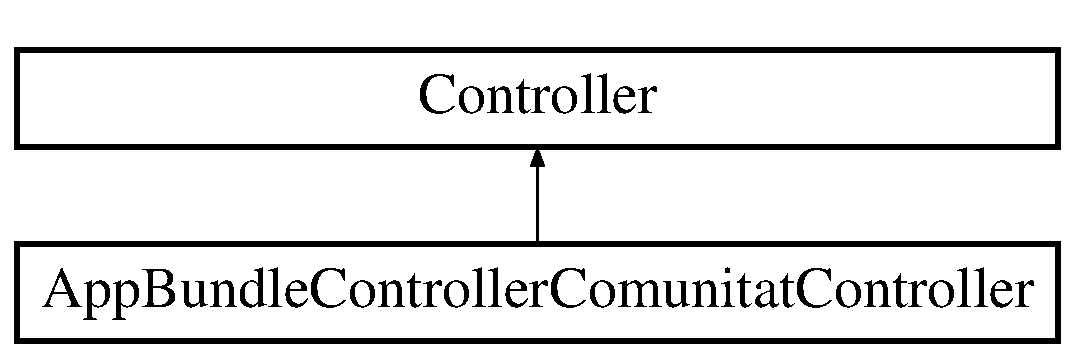
\includegraphics[height=2.000000cm]{class_app_bundle_1_1_controller_1_1_comunitat_controller}
\end{center}
\end{figure}
\subsection*{Public Member Functions}
\begin{DoxyCompactItemize}
\item 
\mbox{\hyperlink{class_app_bundle_1_1_controller_1_1_comunitat_controller_a54cf6158ce22df4010684dd37f98d70c}{principal\+Action}} (Request \$request)
\item 
\mbox{\Hypertarget{class_app_bundle_1_1_controller_1_1_comunitat_controller_adec93957e425d37e1604d2bd46cb3017}\label{class_app_bundle_1_1_controller_1_1_comunitat_controller_adec93957e425d37e1604d2bd46cb3017}} 
{\bfseries noticiaverification\+Action} (Request \$request)
\item 
\mbox{\Hypertarget{class_app_bundle_1_1_controller_1_1_comunitat_controller_ad9b2e6905cc977518c2065e30aef25fb}\label{class_app_bundle_1_1_controller_1_1_comunitat_controller_ad9b2e6905cc977518c2065e30aef25fb}} 
{\bfseries getnoticia} (\$community\+ID)
\item 
\mbox{\Hypertarget{class_app_bundle_1_1_controller_1_1_comunitat_controller_a6cf3f7cfec53fdb8c5e0be4779246f05}\label{class_app_bundle_1_1_controller_1_1_comunitat_controller_a6cf3f7cfec53fdb8c5e0be4779246f05}} 
{\bfseries setnoticia} (\$user\+ID, \$messages, \$img\+Route, \$imgalt=null)
\item 
\mbox{\Hypertarget{class_app_bundle_1_1_controller_1_1_comunitat_controller_a0d529fdcc2dd3d0c72a64804cf8881b0}\label{class_app_bundle_1_1_controller_1_1_comunitat_controller_a0d529fdcc2dd3d0c72a64804cf8881b0}} 
{\bfseries gestio\+Action} (Request \$request)
\item 
\mbox{\Hypertarget{class_app_bundle_1_1_controller_1_1_comunitat_controller_a5d57ea5d895a2e155621411c278f874c}\label{class_app_bundle_1_1_controller_1_1_comunitat_controller_a5d57ea5d895a2e155621411c278f874c}} 
{\bfseries gestio\+Noticies\+Action} (Request \$request)
\item 
\mbox{\Hypertarget{class_app_bundle_1_1_controller_1_1_comunitat_controller_a528f3fb0536e379ef17f399680cde330}\label{class_app_bundle_1_1_controller_1_1_comunitat_controller_a528f3fb0536e379ef17f399680cde330}} 
{\bfseries savefile} (\$file, \$destino)
\end{DoxyCompactItemize}


\subsection{Detailed Description}
Aquesta classe,\mbox{\hyperlink{class_app_bundle_1_1_controller_1_1_comunitat_controller}{Comunitat\+Controller}} s\textquotesingle{}utilitza per a enmagatzemar i controlar totes les funcions i accions que tenen relació amb la comunitat.

Aquesta classe hereda elements de la classe controller que és la classe què contè els elements fonamentals de tots els $\ast$conroladors.

\begin{DoxyAuthor}{Author}
Jordi Herranz Cruz 
\end{DoxyAuthor}


\subsection{Member Function Documentation}
\mbox{\Hypertarget{class_app_bundle_1_1_controller_1_1_comunitat_controller_a54cf6158ce22df4010684dd37f98d70c}\label{class_app_bundle_1_1_controller_1_1_comunitat_controller_a54cf6158ce22df4010684dd37f98d70c}} 
\index{App\+Bundle\+::\+Controller\+::\+Comunitat\+Controller@{App\+Bundle\+::\+Controller\+::\+Comunitat\+Controller}!principal\+Action@{principal\+Action}}
\index{principal\+Action@{principal\+Action}!App\+Bundle\+::\+Controller\+::\+Comunitat\+Controller@{App\+Bundle\+::\+Controller\+::\+Comunitat\+Controller}}
\subsubsection{\texorpdfstring{principal\+Action()}{principalAction()}}
{\footnotesize\ttfamily App\+Bundle\textbackslash{}\+Controller\textbackslash{}\+Comunitat\+Controller\+::principal\+Action (\begin{DoxyParamCaption}\item[{Request}]{\$request }\end{DoxyParamCaption})}

Aquesta funció s\textquotesingle{}utilitza com una acció en escriure la ruta /comunitat/ i retorna la vista que es troba a comunitat/principal.\+html.\+twig a la carpeta views. també retorna un array que conté la ruta per a la gestió


\begin{DoxyParams}{Parameters}
{\em array} & (que conté la ruta d\textquotesingle{}una de les pesstanyes ddel menú)\\
\hline
\end{DoxyParams}
\begin{DoxyAuthor}{Author}
Jordi Herranz Cruz 
\end{DoxyAuthor}


The documentation for this class was generated from the following file\+:\begin{DoxyCompactItemize}
\item 
Comunitat\+Controller.\+php\end{DoxyCompactItemize}

\hypertarget{class_app_bundle_1_1_controller_1_1_perfil_controller}{}\section{App\+Bundle\textbackslash{}Controller\textbackslash{}Perfil\+Controller Class Reference}
\label{class_app_bundle_1_1_controller_1_1_perfil_controller}\index{App\+Bundle\textbackslash{}\+Controller\textbackslash{}\+Perfil\+Controller@{App\+Bundle\textbackslash{}\+Controller\textbackslash{}\+Perfil\+Controller}}
Inheritance diagram for App\+Bundle\textbackslash{}Controller\textbackslash{}Perfil\+Controller\+:\begin{figure}[H]
\begin{center}
\leavevmode
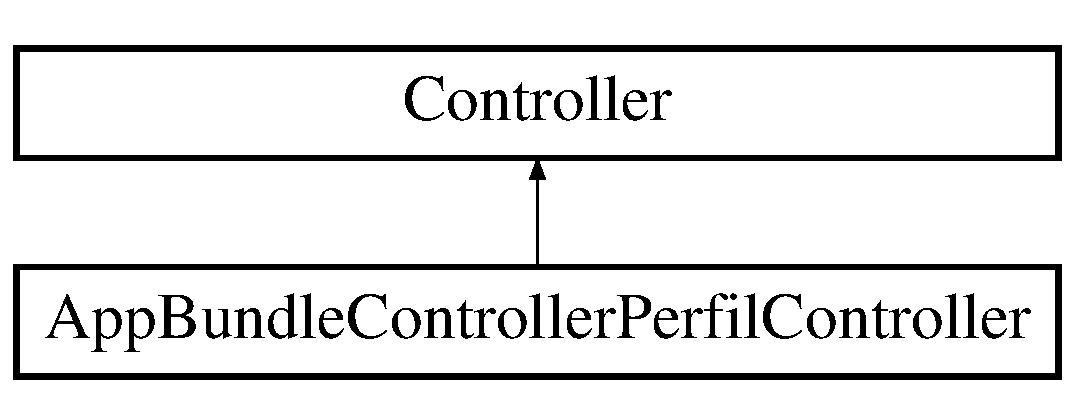
\includegraphics[height=2.000000cm]{class_app_bundle_1_1_controller_1_1_perfil_controller}
\end{center}
\end{figure}
\subsection*{Public Member Functions}
\begin{DoxyCompactItemize}
\item 
\mbox{\Hypertarget{class_app_bundle_1_1_controller_1_1_perfil_controller_a7e36247a985d0625c5b6d8ea6879521a}\label{class_app_bundle_1_1_controller_1_1_perfil_controller_a7e36247a985d0625c5b6d8ea6879521a}} 
{\bfseries perfil\+Action} (Request \$request)
\item 
\mbox{\Hypertarget{class_app_bundle_1_1_controller_1_1_perfil_controller_ac5f66db8ed52f11de13e915611f60eef}\label{class_app_bundle_1_1_controller_1_1_perfil_controller_ac5f66db8ed52f11de13e915611f60eef}} 
{\bfseries postverification\+Action} (Request \$request)
\item 
\mbox{\Hypertarget{class_app_bundle_1_1_controller_1_1_perfil_controller_adc2a62454d2de0f25f2c38066cdcb0c3}\label{class_app_bundle_1_1_controller_1_1_perfil_controller_adc2a62454d2de0f25f2c38066cdcb0c3}} 
{\bfseries gestiouserverification1\+Action} (Request \$request)
\item 
\mbox{\Hypertarget{class_app_bundle_1_1_controller_1_1_perfil_controller_a5823a5118154765161b3d853fab610e2}\label{class_app_bundle_1_1_controller_1_1_perfil_controller_a5823a5118154765161b3d853fab610e2}} 
{\bfseries gestiouserverification2\+Action} (Request \$request)
\item 
\mbox{\Hypertarget{class_app_bundle_1_1_controller_1_1_perfil_controller_a7936c97c37f8547df35c110ac69327ce}\label{class_app_bundle_1_1_controller_1_1_perfil_controller_a7936c97c37f8547df35c110ac69327ce}} 
{\bfseries getpostdatas} (\$user\+ID)
\item 
\mbox{\Hypertarget{class_app_bundle_1_1_controller_1_1_perfil_controller_a50f7a2a6fc226360d3ecfeebbdc5b411}\label{class_app_bundle_1_1_controller_1_1_perfil_controller_a50f7a2a6fc226360d3ecfeebbdc5b411}} 
{\bfseries setpostdatas} (\$user\+ID, \$messages, \$img\+Route, \$imgalt=null)
\item 
\mbox{\Hypertarget{class_app_bundle_1_1_controller_1_1_perfil_controller_a944f6bcd563daa98d04cd2bd616fab57}\label{class_app_bundle_1_1_controller_1_1_perfil_controller_a944f6bcd563daa98d04cd2bd616fab57}} 
{\bfseries savefile} (\$file, \$destino)
\item 
\mbox{\Hypertarget{class_app_bundle_1_1_controller_1_1_perfil_controller_ae2bf2b8b70bacf3a5ab0a30c6b8677ab}\label{class_app_bundle_1_1_controller_1_1_perfil_controller_ae2bf2b8b70bacf3a5ab0a30c6b8677ab}} 
{\bfseries gestiouser\+Action} (Request \$request)
\end{DoxyCompactItemize}


The documentation for this class was generated from the following file\+:\begin{DoxyCompactItemize}
\item 
Perfil\+Controller.\+php\end{DoxyCompactItemize}

\hypertarget{class_app_bundle_1_1_controller_1_1_user_controller}{}\section{App\+Bundle\textbackslash{}Controller\textbackslash{}User\+Controller Class Reference}
\label{class_app_bundle_1_1_controller_1_1_user_controller}\index{App\+Bundle\textbackslash{}\+Controller\textbackslash{}\+User\+Controller@{App\+Bundle\textbackslash{}\+Controller\textbackslash{}\+User\+Controller}}
Inheritance diagram for App\+Bundle\textbackslash{}Controller\textbackslash{}User\+Controller\+:\begin{figure}[H]
\begin{center}
\leavevmode
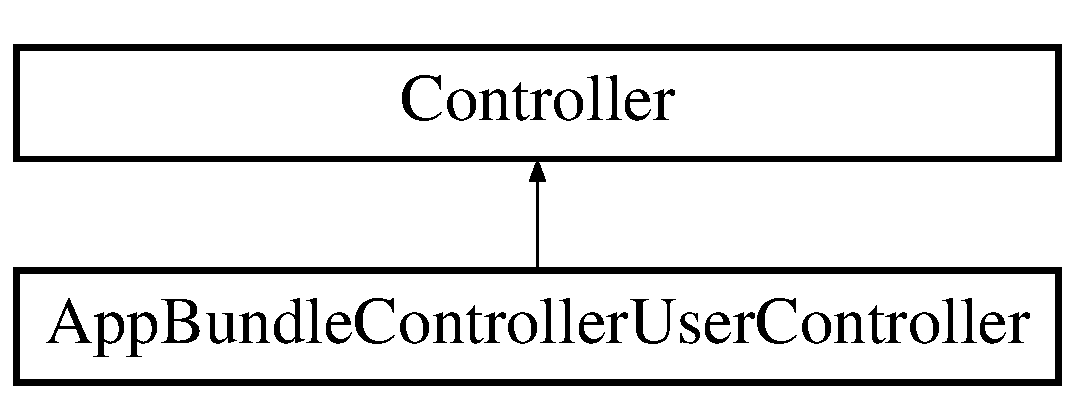
\includegraphics[height=2.000000cm]{class_app_bundle_1_1_controller_1_1_user_controller}
\end{center}
\end{figure}
\subsection*{Public Member Functions}
\begin{DoxyCompactItemize}
\item 
\mbox{\hyperlink{class_app_bundle_1_1_controller_1_1_user_controller_a268cbed26597ca6ca90c00b8a2bcd0c9}{loginverification\+Action}} (Request \$request)
\item 
\mbox{\Hypertarget{class_app_bundle_1_1_controller_1_1_user_controller_ac888ff4055820cfce7a3848b1883b722}\label{class_app_bundle_1_1_controller_1_1_user_controller_ac888ff4055820cfce7a3848b1883b722}} 
{\bfseries registreverification\+Action} (Request \$request)
\item 
\mbox{\Hypertarget{class_app_bundle_1_1_controller_1_1_user_controller_a0605acce42e82bd54b64833480b0f115}\label{class_app_bundle_1_1_controller_1_1_user_controller_a0605acce42e82bd54b64833480b0f115}} 
{\bfseries login\+Action} (Request \$request)
\item 
\mbox{\Hypertarget{class_app_bundle_1_1_controller_1_1_user_controller_a42dd961822df9f7eba01f82b8fd2df30}\label{class_app_bundle_1_1_controller_1_1_user_controller_a42dd961822df9f7eba01f82b8fd2df30}} 
{\bfseries searchresult\+Action} (Request \$request)
\item 
\mbox{\Hypertarget{class_app_bundle_1_1_controller_1_1_user_controller_a3f5df2466aaf1e84b63c32a9f4fd524e}\label{class_app_bundle_1_1_controller_1_1_user_controller_a3f5df2466aaf1e84b63c32a9f4fd524e}} 
{\bfseries generaresult} (\$object\+\_\+array, \$tip)
\end{DoxyCompactItemize}


\subsection{Member Function Documentation}
\mbox{\Hypertarget{class_app_bundle_1_1_controller_1_1_user_controller_a268cbed26597ca6ca90c00b8a2bcd0c9}\label{class_app_bundle_1_1_controller_1_1_user_controller_a268cbed26597ca6ca90c00b8a2bcd0c9}} 
\index{App\+Bundle\+::\+Controller\+::\+User\+Controller@{App\+Bundle\+::\+Controller\+::\+User\+Controller}!loginverification\+Action@{loginverification\+Action}}
\index{loginverification\+Action@{loginverification\+Action}!App\+Bundle\+::\+Controller\+::\+User\+Controller@{App\+Bundle\+::\+Controller\+::\+User\+Controller}}
\subsubsection{\texorpdfstring{loginverification\+Action()}{loginverificationAction()}}
{\footnotesize\ttfamily App\+Bundle\textbackslash{}\+Controller\textbackslash{}\+User\+Controller\+::loginverification\+Action (\begin{DoxyParamCaption}\item[{Request}]{\$request }\end{DoxyParamCaption})}

(\char`\"{}/\char`\"{}, name=\char`\"{}homepage\char`\"{}) 

The documentation for this class was generated from the following file\+:\begin{DoxyCompactItemize}
\item 
User\+Controller.\+php\end{DoxyCompactItemize}

%--- End generated contents ---

% Index
\backmatter
\newpage
\phantomsection
\clearemptydoublepage
\addcontentsline{toc}{chapter}{Index}
\printindex

\end{document}
